% !TEX root = ../main.tex

\section{Determination of Extraction Conditions} % (fold)
\label{sec:determination_of_extraction_conditions}

% section determination_of_extraction_conditions (end)

\section{Chromatographic Separation} % (fold)
\label{sec:chromatographic_separation}

    \subsection{Reverse-Phase HPLC} % (fold)
    \label{sub:reverse_phase_hplc}

    % subsection reverse_phase_hplc (end)

    \subsection{HPLC with Amino Column} % (fold)
    \label{sub:hplc_with_amino_column}

    % subsection hplc_with_amino_column (end)

    \subsection{Hydrophilic Interaction Chromatography} % (fold)
    \label{sub:hydrophilic_interaction_chromatography}

    % subsection hydrophilic_interaction_chromatography (end)

    \subsection{Ion exchange Chromatography} % (fold)
    \label{sub:ion_exchange_chromatography}

    % subsection ion_exchange_chromatography (end)

    \subsection{Thin-Layer Chromatography} % (fold)
    \label{sub:thin_layer_chromatography}

    % subsection thin_layer_chromatography (end)

% section chromatographic_separation (end)

\section{Dereplication} % (fold)
\label{sec:dereplication}

    \subsection{HPLC Mass Spectrometry} % (fold)
    \label{sub:hplc_mass_spectrometry}

    % subsection hplc_mass_spectrometry (end)

    \subsection{Trimethylsilane Derivatization and Gas Chromatography} % (fold)
    \label{sub:trimethylsilane_derivatization_and_gas_chromatography_results}

    % subsection trimethylsilane_derivatization_and_gas_chromatography (end)

% section dereplication (end)

\section{Antibacterial Activity Spectrum} % (fold)
\label{sec:antibacterial_activity_spectrum}


    \subsection{Activity against E. coli} % (fold)
    \label{sub:activity_against_e_coli}

    % subsection activity_against_e_coli (end)

    \subsection{Activity against B. subtilis} % (fold)
    \label{sub:activity_against_b_subtilis}

    % subsection activity_against_b_subtilis (end)

    \subsection{Extraction of yorB-inducing Compound} % (fold)
    \label{sub:extraction_of_yorb_inducing_compound}

%    Tü2401 displayed positive results in the yorB-Assay \todo{Referenz einsetzen} when grown on ISP2 plates \todo{Referenz einsetzen}. However, all previously generated samples from liquid cultures only showed antibacterial activity.
%    %%%%%%%%%%%%%%
%    %Einsetzen:
%    %%%%%%%%%%%%%%
%    % Absatz über Differenzierung von Streptomyceten
%    % Einfluss auf Sekundärmetabolismus
%    % Überleitung zu Schlussfolgerung: Evtl zweiter Compound nur auf agar produziert
%    %%%%%%%%%%%%%%%
%    Three cultivation strategies were developed to induce production of the putative compound 2 (PC2):
%
%    \begin{enumerate}
%        \item Standing cultures could allow the formation of aerial mycelium at the medium surface. Thus, enabling the synthesis of PC2 and allowing extraction of the liquid medium. Two \SI{500}{\milli\liter} flasks were each filled with \SI{100}{\milli\liter} of liquid ISP2 medium and inoculated with \SI{1}{\milli\liter} of a one-week old NL~410 shake culture. One flask was sealed with an ordinary aluminium cap (AC), the other one with an air-permeable foam cap (FC). Both flasks were cultivated for four days, before the medium was centrifuged and the supernatant filtrated. \SI{50}{\milli\liter} aliquots of each flask were extracted with either BuOH or EtAc, and both phases were collected seperately. The organic phases were dried at \SI{40}{\celsius} and solved in \SI{1}{\milli\liter} MeOH. Both phases of each flask were subjected to the yorB-Assay.
%        \item ISP2 agar plates were previously known to enable synthesis of PC2 and could be extracted with prior breakup. Ten round ISP2 agar plates were inoculated with \SI{100}{\micro\liter} of a one-week old NL~410 shake culture and incubated for four days. One half of the plates was extracted with BuOH, the other half was extracted with EtAc.
%        \item ISP2 agar plates could also be prepared with low-melting-point agarose (LMPA). This would allow melting of the plates at lower temperatures. Thus, allowing for easier extraction with reduced risk of thermal decomposition during the process. Six ISP2 LMPA agar plates were inoculated with \SI{100}{\micro\liter} of a week-old NL~410 shake culture and incubated for four days. The plates were then melted at \SI{70}{\celsius} and extracted with BuOH and EtAc.
%    \end{enumerate}
%
%    All generated extracts and their respective aqueous phases were tested for bioactivity. The standard bioassay was used to determine the antibiotic activity against \textit{E. coli} K12 and \textit{B. subtilis} 168, and the yorB-Assay was used to test for the mode of action. Additonally, agar stamps of grown ISP2 and ISP2 LMPA plates were tested in the yorB-Assay. A summary of the results is shown in \todo{Tabelle einsetzen}.
%
%    \begin{table}[htbp]
%        \caption[Bioassay results from agar-plate and standing culture extraction]{\textbf{Bioassay results from agar-plate and standing culture extraction}.\\
%        Samples were screened for antibiotic activity against \textit{E. coli} K12 and \textit{B. subtilis} 168 and for promotor induction in the yorB-Assay.
%        Samples from standing cultures with foam cap (FC) or aluminium cap (AC), ISP2 agar plates (ISP2) and ISP2 agar plates with low-melting-point agarose (LMPA). Samples were extracted with butanol (BuOH) or ethyl acetate (EtAc) and tested alongside their respective aqueous phases (aq.). \emph{Legend}: \textbf{-} No activity; \textbf{+ / ++ / +++} antibiotic activity with inhibition zone of 1~/~1.0-1.5~/~>1.5~cm; \textbf{n.e.} result non-evaluable}
%        \label{tab:yorB_assay_results}
%        \centering
%        \begin{tabularx}{\textwidth}{XXXXX}
%            \toprule
%            & \multicolumn{3}{c}{Antibacterial} & positive \\
%            \cline{2-4}
%            \textbf{Sample} & \textbf{\textit{E. coli}}     & \textbf{\textit{B. subtilis}}  & \textbf{yorB}  & \textbf{yorB}    \\
%            \midrule
%            FC BuOH         & -     & -     & -     & -    \\
%            FC BuOH aq.     & -     & -     & -     & -    \\
%            FC EtAc         & -     & +++   & ++    & -    \\
%            FC EtAc aq.     & -     & -     & -     & -    \\
%            AC BuOH         & -     & -     & -     & -    \\
%            AC BuOH aq.     & -     & -     & -     & -    \\
%            AC EtAc         & -     & -     & +     & -    \\
%            AC EtAc aq.     & -     & -     & -     & -    \\
%            ISP2 BuOH       & -     & n.e.  & +++   & -    \\
%            ISP2 BuOH aq.   & -     & +     & -     & -    \\
%            ISP2 EtAc       & -     & ++    & -     & -    \\
%            ISP2 EtAc aq.   & +     & n.e.  & -     & +    \\
%            ISP2 plaque     &       &       & ++    & ++   \\
%            LMPA BuOH       & +     & n.e.  & +++   & -    \\
%            LMPA BuOH aq.   & -     & n.e.  & -     & -    \\
%            LMPA EtAc       & -     & n.e.  & +++   & -    \\
%            LMPA EtAc aq.   & -     & n.e.  & -     & -    \\
%            LMPA plaque     &       &       & ++    & ++   \\
%            \bottomrule
%        \end{tabularx}
%    \end{table}
    % subsection extraction_of_yorb_inducing_compound (end)

% section antibacterial_activity_spectrum (end)

\section{Genomic Analysis} % (fold)
\label{sec:genomic_analysis}

    \subsection{Phylogeny of Strain Tü2401} % (fold)
    \label{sub:phylogeny_of_strain_tue2401}

	\begin{figure}[htbp]
		\label{fig:phylo_tree}
		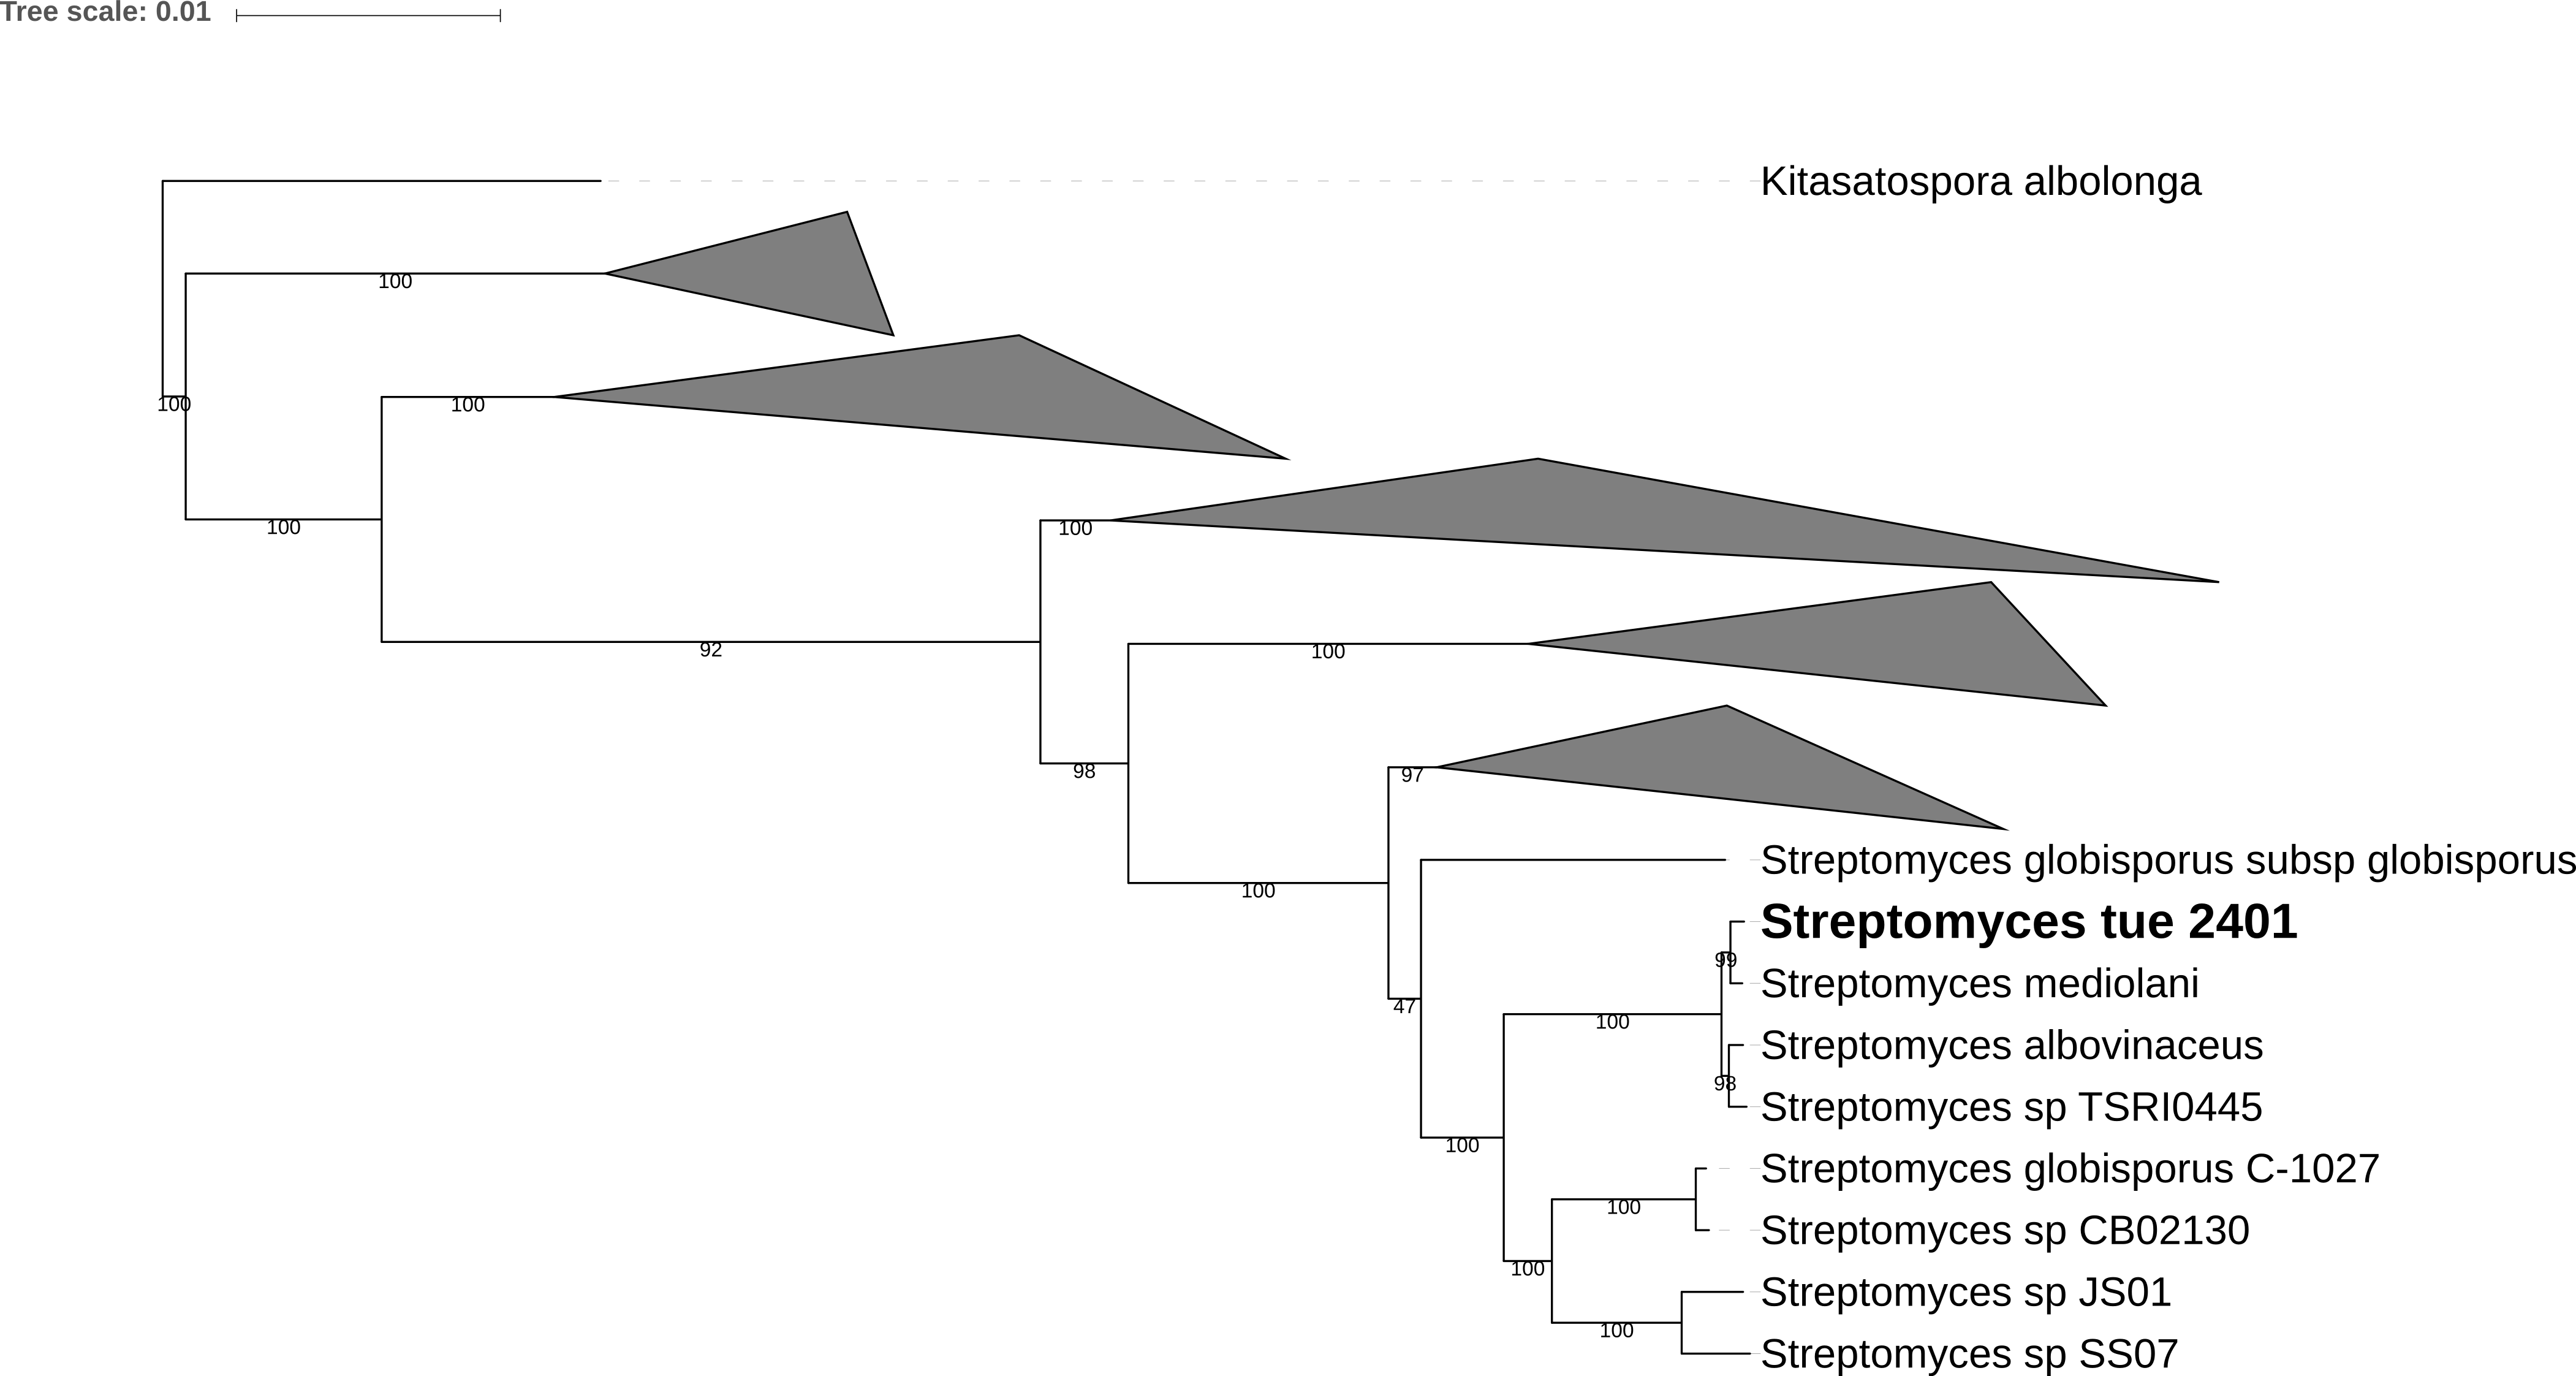
\includegraphics[width=\textwidth]{tu2401_tree}
		\caption[Maximum likelihood tree of \emph{Streptomyces} sp. Tü2401.]{\textbf{Maximum likelihood tree of \emph{Streptomyces} sp. Tü2401.}} 
	\end{figure}

    % subsection phylogeny_of_strain_tü2401 (end)

    \subsection{AntiSMASH Cluster Identification} % (fold)
    \label{sub:antismash_cluster_identification}

	 One cluster was detected on contig four and identified as a Type1-PKS-NRPS hybrid. It shows a 95~\% cluster identity to the C-1027 biosynthetic gene cluster from \textit{Streptomyces} globisporus C-1027 (MiBiG accession no. BGC0000965). Additionally, three homologous subclusters with 100~\% identity were identified, which are associated with the synthesis of C-1027, Neocarzinostatin and Maduropeptin enediynes (see Figure \ref{fig:cluster_search}).The presence of this cluster could indicate, that the strain Tü2401 is capable of producing a compound similar to enediyne antibiotics. 
	 
	 Enediyne natural products are a class of cytotoxic bacterial compounds, which cause extensive DNA-damage.\autocite{Liang2010,Gredicak2007,AdrianL.Smith*1996,Nicolaou1993} 11 different enediyne natural products are known, all of which feature either a bicyclo[7.3.0]dodecadienediyne core inside a nine-membered ring or a bicyclo[7.3.1]tridecadiynene core inside a ten-membered ring (Figure \ref{fig:enediyne_comparison}). The 9-membered family includes neocarzinostatin, C-1027 and and maduropeptin. The 10-membered family includes calicheamicin $\gamma_{1}^{I}$, esperamicin A\textsubscript{1} and dynemicin A. \autocite{Liang2010} Enediynes are potent cytotoxic agents because of their ability to induce DNA double-strand breaks.\autocite{Shen2015} Electronic rearrangement of the carbocycle produces a benzenoid diradical, which abstracts hydrogen atoms from the DNA-backbone. The consulting radicals cause interstrand crosslinks or react with molecular oxygen.	 
	 \begin{figure}[htbp]
	 	\label{fig:enediyne_comparison}
	 	\centering
	 	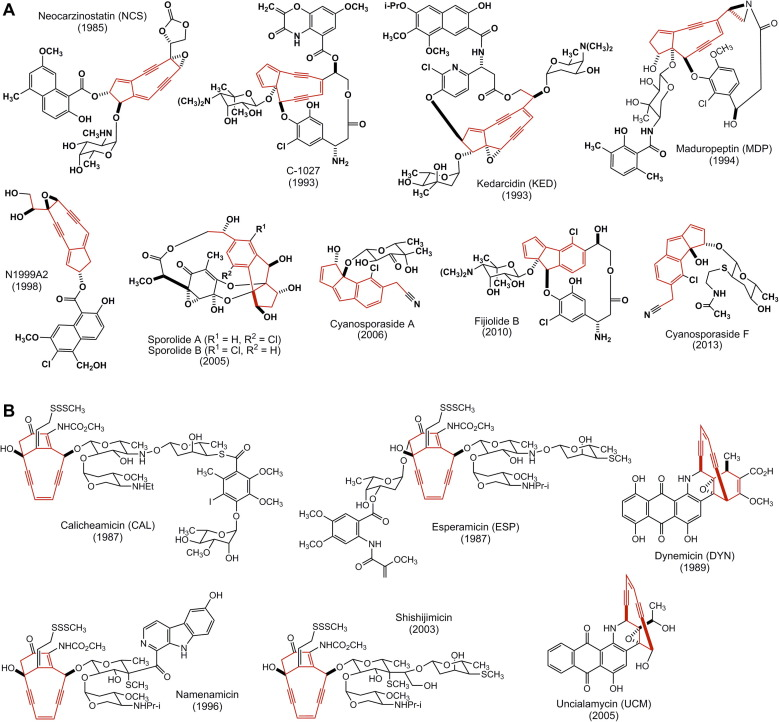
\includegraphics[width=0.9\textwidth]{enediyne_overview}
	 	\caption[Structures of known enediyne natural products]{\textbf{Structures of known enediyne natural products.} Enediyne cores are highlighted in red. (A) Compounds with nine-membered rings. (B) Compounds with ten-membered rings. The year of structure confirmation is displayed in parentheses. The sporolides, cyanosporolids and fijiolides do not contain an endiyene core, but are proposed to be derived from enediyne precursors. Reprinted from Shen \textit{et al.} (2015) Copyright 2014 Elsevier Ltd.}
	 \end{figure}
	 While the ten-membered enediyne compounds were isolated as free-standing chromophores, most of the compounds in the nine-membered family were isolated in conjunction with a protective apoprotein.\autocite{Liang2010} The nine-membered chromophore of C-1027, which was isolated from \textit{Streptomyces} globisporus C-1027, is bound noncovalently to an 110 amino acid apoprotein.\autocite{AdrianL.Smith*1996,Minami1993,Yoshida1993,Otani1993,Sugiura1993,Matsumoto1993,Otani1991,Otani1988a,Matsumoto1993a} The isolated chromophore has been shown to be very unstable, whereas the holo C-1027 did not lose activity under the same conditions. \autocite{Matsumoto1993,Sugiura1993,Otani1991} The apoprotein binds specifically to the C-1027 chromophore, supposedly by hydrophic pocket, which binds the benzoxazine side chain. \autocite{Okuno1994,Matsumoto1993} The enediyne antibiotics neocarzinostatin and maduropeptin, which were also isolated from actinomycetes, also feature highly specific and protective apoproteins. \autocite{AdrianL.Smith*1996}.
	 
	 The homologies of the identified cluster could be an indicator, that the strain Tü2401 is capable of synthesizing an enediyene antibiotic with a nine-membered core and a corresponding apoprotein. The potent DNA-strand-breaking capabilities of this compound-class could induce the \textit{yorB} reporter system of \textit{Bacillus subtilis} 1S34 pHJS105-yorB-lacZ2 in the yorB-induction assay. A number of compounds, which cause DNA double strand breaks and crosslinks are reported to induce the system, though none of them belong to the family of endiyne antibiotics. \autocite{Urban2007} Whether this is due to inactivity or to this family not having been tested in the assay is unclear, since the compound library is not publicly accessible. Nevertheless, an endiyne compound could be responsible for the induction.
	 
	 The assay in Section \ref{sub:extraction_of_yorb_inducing_compound} showed, that the \textit{yorB} inducing compound is produced when the strain is grown on an ISP2 agar plate, but it could not be extracted via ethyl acetate or butanol. Only very low activity was retained in the aqueous phase. If the compound is indeed an endiyne, this loss of activity could be due to the high instability of the chromophore. The apoprotein could have been detached during the extraction and concentration process, which also included high temperatures of \SIrange[range-units=single]{40}{60}{\celsius}. Combined with an incubation time of several days between extraction and assay, this could have led to the degradation of the chromophore below the sensitivity threshhold. The high temperatures and long storage times also apply to the numerous HPLC-fractioning samples subjected to the \textit{yorB}-induction assay. 
	 
	 To verify this assumption, the putative endiyne compound has to be extracted by an adapted protocol, dereplicated and subjected to the assay in pure form. The C-1027 antibiotic protein from \textit{S. globisporus} was precipitated from the medium supernatant by the addition of ammonium sulfate and purified by dialysis and column chromatography.\autocite{Otani1988a} The active chromophore could be extracted from the apoprotein with methanol at \SI{0}{\celsius}. \autocite{Matsumoto1993} However, as of now, untreated medium supernatant samples of the strain Tü2401 did not induce the \textit{yorB}-reporter system. The cultivation in liquid OM medium is probably not sufficient for production of the putative endiyene compound and the protocol would have to be adapted for the extraction from ISP2 agar plates. To circumvent this, other cultivation media could be employed and tested for \textit{yorB}-induction. The holo endiyne-apoprotein complex should be stable enough for routine testing of media and media supernatants. The only alternative to optimizing production conditions would be heterologous expression of the biosynthetic cluster. For the endiyne compound family though, this has, as of now, only been partly achieved for the nine-membered endiyne neocarzinostatin.\autocite{Zhang2008}
	 
	 The isolation of the putative endiyne antibiotic would be a very promising target. Only eleven compounds of this class are known to this date, yet several members are in use or development as anticancer drugs with promising results.\autocite{Liang2010,Galm2005} Isolation of a new endiyne compound could  hold a strong promise for the discovery of a new anticancer drug lead structure.
	 
    % subsection antismash_cluster_identification (end)

% section genomic_analysis (end)

